\section{Direct fault injection into the classical stage}
\label{sec:adversarial}

Sweeps perturb inputs; this section perturbs the reconstruction stage
itself, injecting five conditions at 32 trials each
(Fig.~\ref{fig:adversarial}).

Three conditions leave the outcome untouched at $100\%$: a clean control, a
post-hoc bit flip, and the insertion of an incorrect high-weight candidate.
The stitching stage rejects or out-ranks all three. Removing the true
candidate from a window drops success to $78.1\%$ --- not to zero, because
overlap redundancy can still recover the phase from the remaining windows.
Corrupting an overlap region is the only severe condition, at $43.8\%$.

That last figure was originally attributed to the carry-aware consistency
check being over-permissive. Section~\ref{sec:retraction} reports why that
attribution was wrong, and what the correct one is.

\begin{figure}[htbp]
\centering
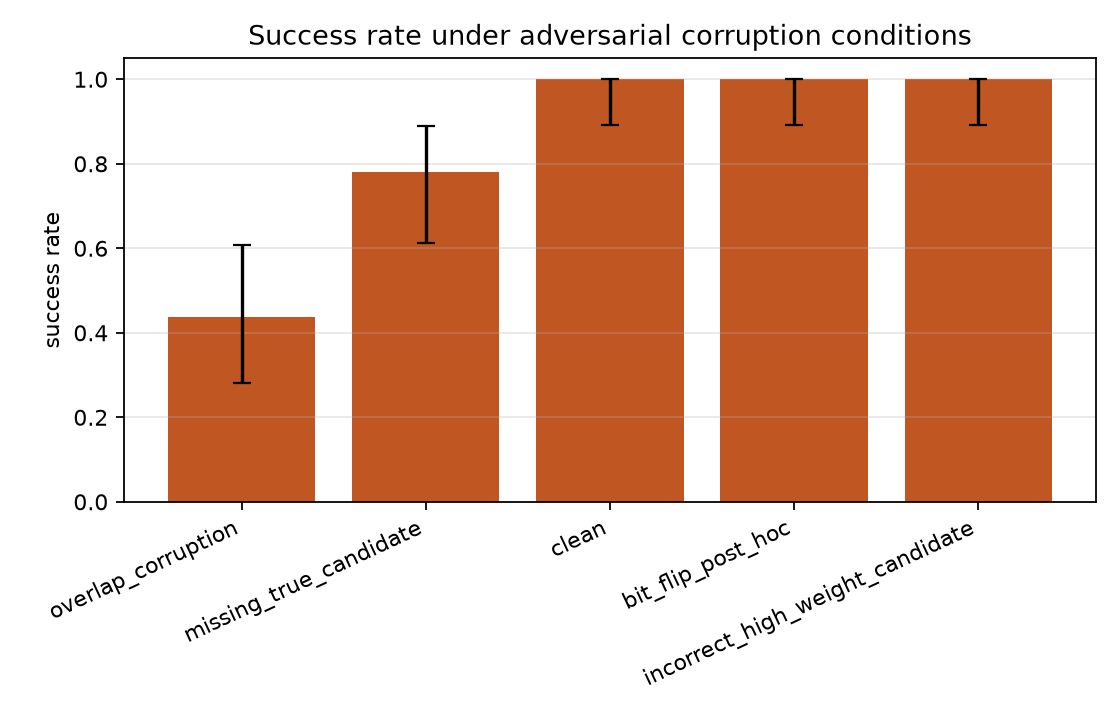
\includegraphics[width=0.78\linewidth]{../Data/failure_study/plots/adversarial_conditions.png}
\caption{\textbf{End-to-end success under direct fault injection}, 32 trials
per condition. The reconstruction logic absorbs post-hoc bit flips and
misleading high-weight candidates completely. Only overlap corruption is
severe, and Sec.~\ref{sec:retraction} shows the mechanism is budget
starvation rather than a defective consistency check. Rendered from
\texttt{phase3\_adversarial.csv}.}
\label{fig:adversarial}
\end{figure}

\subsection{A sharp instability at the ambiguity boundary}
\label{sec:ambiguity}

One failure mode is sharply defined and is not addressed anywhere in this
article. When a window's true phase sits close to the $0.5$ boundary between
adjacent buckets, the winning bit pattern is unstable across repeated
identical measurements. Table~\ref{tab:ambiguity} locates the transition
precisely: at distance $\delta\le0.005$ from the boundary the winner
disagrees across repeats on \textbf{every} trial, and by $\delta=0.010$ it
disagrees on none.

This is a property of the window geometry, not of the reconstruction budget.
No amount of additional sampling or candidate retention fixes it, because
the two competing patterns are genuinely near-equiprobable. Fixing it
requires revising the window boundaries, which regenerates circuits --- and
is therefore out of scope for a classical post-processing intervention.

\begin{table}[htbp]
\centering\small
\caption{Instability at the bucket boundary, 20 repeated identical
measurements per distance. ``Flagged'' is the fraction a $0.9$ top-share
threshold marks ambiguous; ``winner disagrees'' is the fraction where
repeated identical measurements do not agree on the winning pattern. The
transition is complete within one percentage point of the boundary. From
\texttt{phase3\_ambiguity\_boundary.csv}.}
\label{tab:ambiguity}
\begin{tabular}{@{}lrrrr@{}}
\toprule
$\delta$ from boundary & Top-1 share & 2nd share & Flagged & Winner disagrees \\
\midrule
0.000 & 0.413 & 0.402 & 1.00 & \textbf{1.00} \\
0.001 & 0.412 & 0.401 & 1.00 & \textbf{1.00} \\
0.002 & 0.415 & 0.400 & 1.00 & \textbf{1.00} \\
0.005 & 0.414 & 0.400 & 1.00 & \textbf{1.00} \\
0.010 & 0.423 & 0.391 & 0.80 & 0.00 \\
0.020 & 0.438 & 0.375 & 0.00 & 0.00 \\
0.050 & 0.490 & 0.326 & 0.00 & 0.00 \\
0.100 & 0.571 & 0.255 & 0.00 & 0.00 \\
0.250 & 0.811 & 0.091 & 0.00 & 0.00 \\
\bottomrule
\end{tabular}
\end{table}
